%!TEX root = paper.tex

\section{Discussion on Temperature}
\label{sec:discussion}

It is well known that CFO impairment varies with the temperature. A natural question is how robust is the attack with temperature. In this section, we specifically consider variation in the fingerprint due to temperature and evaluate in detail, if during normal operation does the temperature change significantly. An interesting observation in most typical operating conditions our attack would still work. 

In order to understand the impact of temperature on our attack, we need to understand if CFO and IQ offset are dependent on temperature, and if so how much does that impact our tracking attack.
%
To analyze the temperature dependence, we collect BLE beacons from a Moto G6 phone running an official COVID-19 tracking app. 
%
The phone operational mode is varied significantly, from a typical mode of of phone screen off and several apps running in background over WiFi, to playing heavy-duty game (Asphalt 9) app. During this time, we observe the CFO and IQ variations on a per-packet basis, record the on-board PMIC temperature sensor values during the test, and the ambient temperature during the experiment as a point of reference. 

\begin{comment}
\begin{figure}[t!]
    \centering
    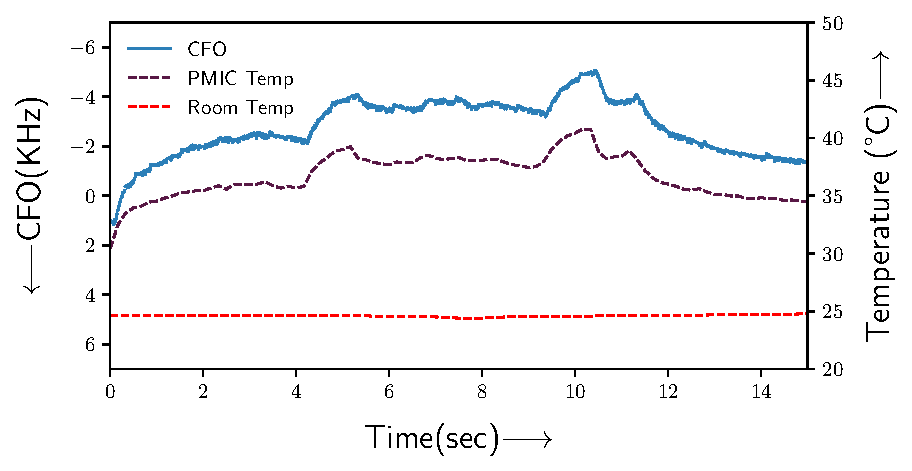
\includegraphics[width = \linewidth]{plots/exert_cfo.pdf} 
    \caption{CFO variation with temperature when playing game}
    \label{fig:exert_cfo}
\end{figure}
\end{comment}
\begin{figure}
    \centering
    \begin{subfigure}[b]{1\linewidth}
       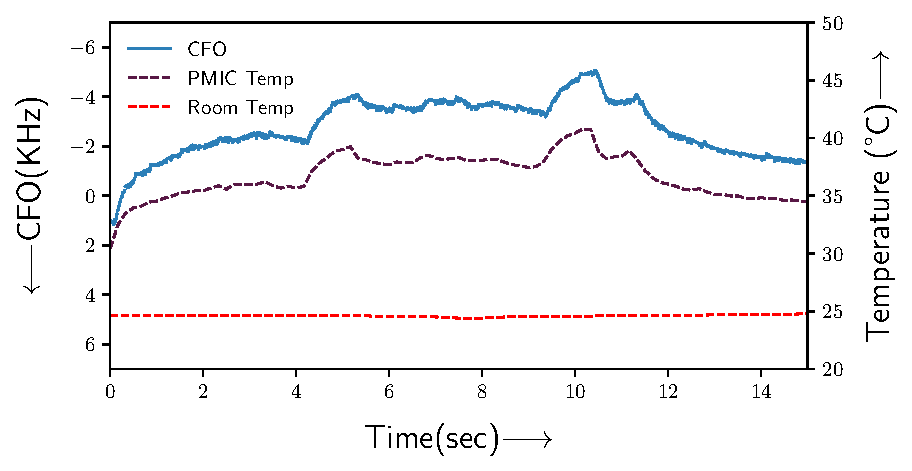
\includegraphics[width=1\linewidth]{plots/exert_cfo.pdf}
       \caption{}
       \label{fig:exertcfo} 
    \end{subfigure}
    
    \begin{subfigure}[b]{1\linewidth}
       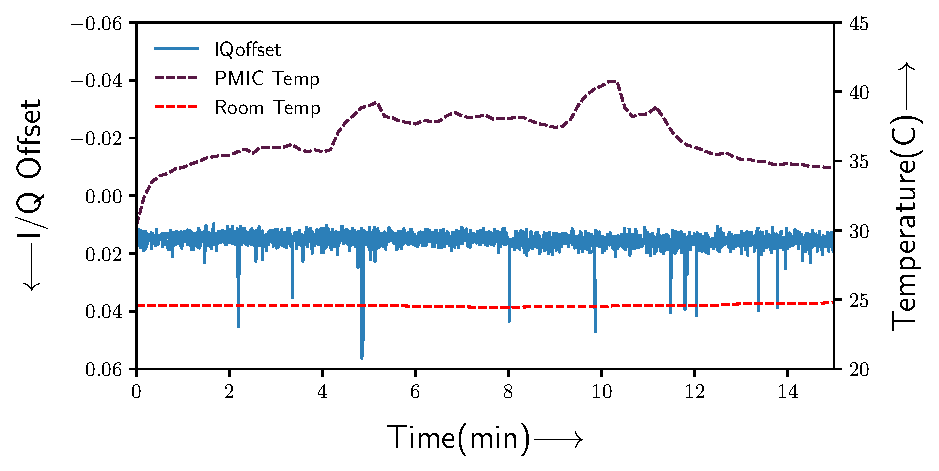
\includegraphics[width=1\linewidth]{plots/exert_iq.pdf}
       \caption{}
       \label{fig:exertiq}
    \end{subfigure}
    
    \caption[Two numerical solutions]{Variation in CFO over time in non-active use cases (a) Phone in pocket (b) Phone on table}
\end{figure}

Figure~\ref{fig:exertcfo} shows the plot of CFO variation during the test, we note that PMIC temperature directly relates to the variation in CFO. 
%
We see that as usage of phone increases it results in a jump in temperature of almost 10 \textdegree C, which results in CFO variation of 6 KHz, but gradual increase, and starts reversing as soon as the activity subsides. Figure.~\ref{fig:exertiq} shows no variation in IQ during the entire experiment making it robust to temperature variation. 
%
Nonetheless, this would impact our tracking mechanism, as CFO is the major contributor.% to identification.


To evaluate the impact in the real-world, we leverage existing studies and experimentation to understand the impact of the variation in the CFO. In the real world people don't continuously use their phones.
%
According to a survey by Rescue Time~\cite{mobileusage}, people spend on average only 3.5 hours per day on the phone, and 70\% of these usages are less than 2 min. 
%
For a majority of the time, our phone is in typical background mode only, i.e., phone screen off, and notifications enabled.
%

To understand how the CFO varies with temperature in background mode, we consider two experiments --- phone with screen off kept on table, and phone kept in pocket.
%
From a user perspective these two situations are similar, but for our attack keeping the phone in pocket close to the skin leads to increase in phone temperature.
%
\begin{figure}
    \centering
    \begin{subfigure}[b]{1\linewidth}
       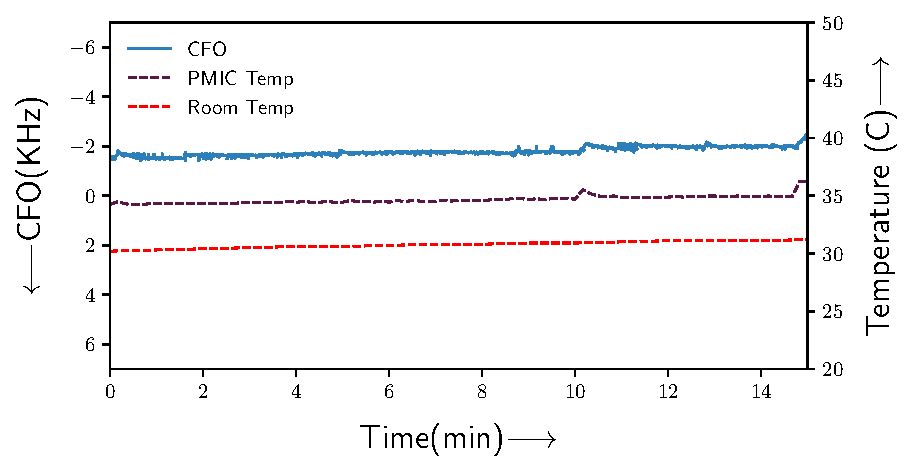
\includegraphics[width=1\linewidth]{plots/pocket_cfo.pdf}
       \caption{}
       \label{fig:pocketcfo} 
    \end{subfigure}
    
    \begin{subfigure}[b]{1\linewidth}
       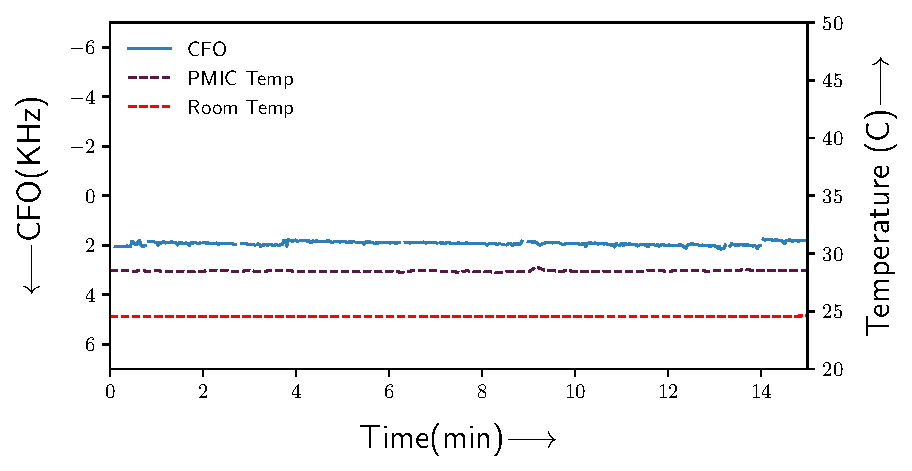
\includegraphics[width=1\linewidth]{plots/table_cfo.pdf}
       \caption{}
       \label{fig:tablecfo1}
    \end{subfigure}
    % \begin{subfigure}[b]{1\linewidth}
    %     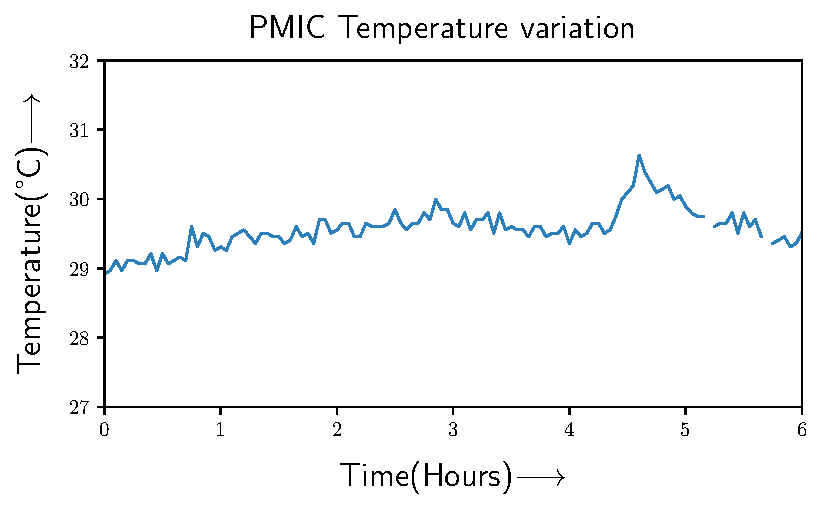
\includegraphics[width=1\linewidth]{plots/pmic_temp_plot.pdf}
    %     \caption{}
    %     \label{fig:tablecfo2}
    %  \end{subfigure}
    \caption[Two numerical solutions]{Variation in CFO over time in non-active use cases (a) Phone in pocket (b) Phone on table}
\end{figure}

Figure.~\ref{fig:pocketcfo} and Figure.~\ref{fig:tablecfo1} shows the variation of CFO during both these situations.
%
We observe the temperature inside the pocket is 5 \textdegree C higher than on the table.
%
Consequently, the CFO is about 3 KHz higher when in the pocket.
%
Interestingly, whether inside the pocket or on the table, the temperature and CFO are very stable.
%
This indicates tracking can be done as long as both fingerprinting and eventual identification are both done in one of the two situations, but not cross scenario, i.e., fingerprint derived on table and tracking performed with device in pocket.
%

Kang et al.~\cite{fireinyourhands} showed that variations in room temperature have minimal thermal impact on mobile phones. Therefore, we expect that a table experiment will result in robust tracking. 
%
To explore how stable temperature inside pocket remains during a long duration of capture, we performed a field experiment to record the PMIC temperature during a 6 hour window.
%
During this time, the volunteer had phone in their pocket and performed typical daily activities like walking to work, sitting and moving around in workspace
%
We observed a maximum variation of only 1.5 \textdegree C in PMIC temperature during this time, which indicates that phone in pocket can also lead to stable CFO values.

\begin{comment}
\begin{figure}
    \centering
    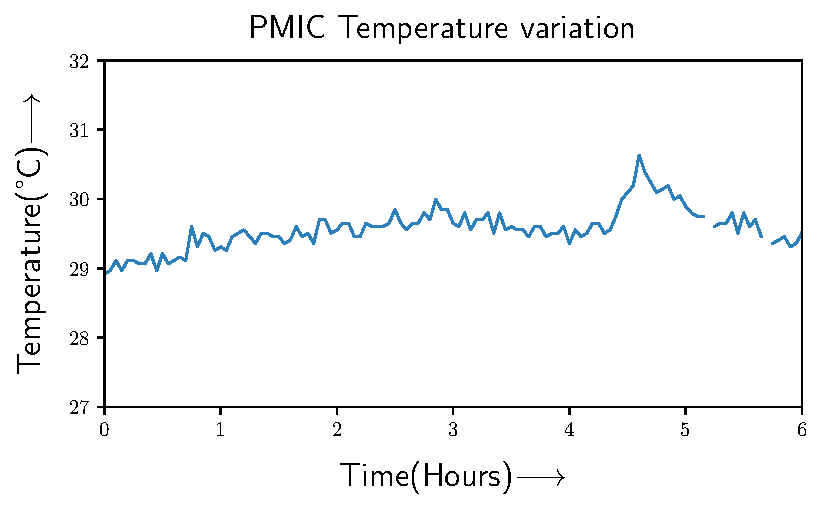
\includegraphics[width = \linewidth]{plots/pmic_temp_plot.pdf} 
    \caption{Variation in PMIC temperature with phone in pocket for long duration}
    \label{fig:pmic_temp_long}
\end{figure}
\end{comment}

\begin{comment}
\begin{figure}
    \centering
    \begin{subfigure}[b]{1\linewidth}
       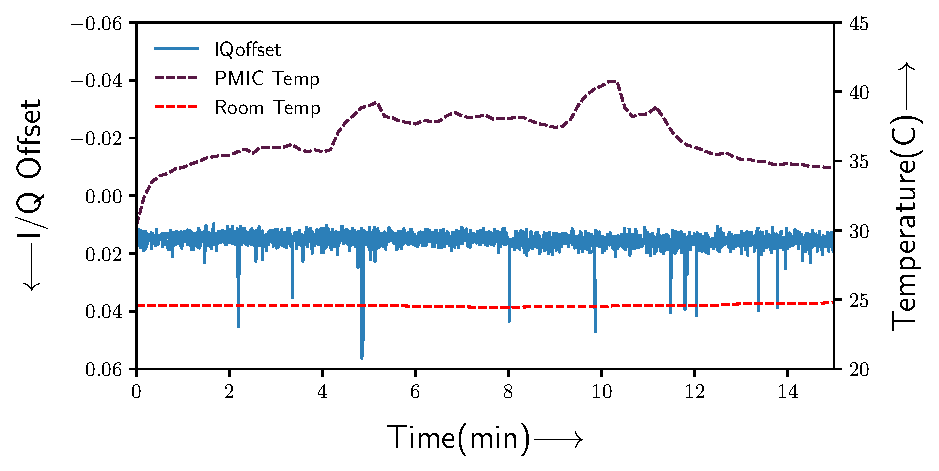
\includegraphics[width=1\linewidth]{plots/exert_iq.pdf}
       \caption{}
       \label{fig:Ng1} 
    \end{subfigure}
    
    \begin{subfigure}[b]{1\linewidth}
       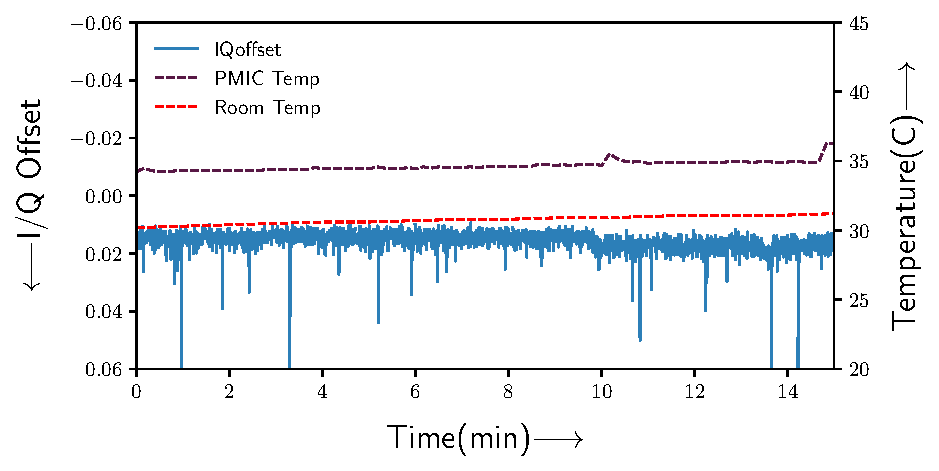
\includegraphics[width=1\linewidth]{plots/pocket_iq.pdf}
       \caption{}
       \label{fig:Ng2}
    \end{subfigure}
    
    \caption[Two numerical solutions]{Variation in IQ offset over time (Dummy figure}
\end{figure}
\end{comment}
To summarize, while temperature variations result in CFO variations, we observe no significant impact on our ability to track individuals. Particularly in the most common usages of mobile devices, stable CFO values can be derived from BLE signals. In addition, IQ offset is independent variation, and future work can utilize this aspect to make this tracking particularly stable across wide variety of conditions.


\begin{comment}
\begin{figure}[t!]
    \centering
    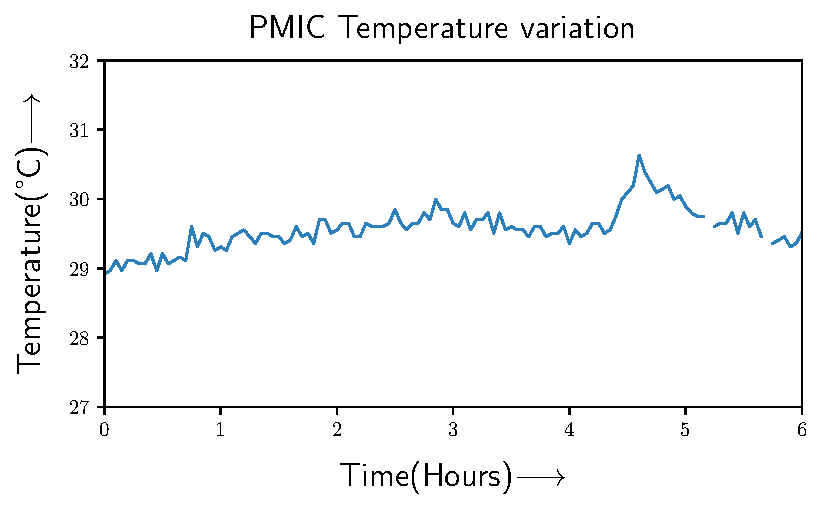
\includegraphics[width = \linewidth]{plots/pmic_temp_plot.pdf} 
    \caption{CFO Comparison of two SDRs (Dummy)}
    \label{fig:pmic_temp_long}
\end{figure}
\end{comment}
\begin{comment}

\noindent\textbf{Temperature:}
\\
Electronic devices can have varying temperature depending on ambient conditions, and device activity
%
Temperature changes cause variation in frequency output of crystal oscillators, resulting in change of CFO.
%

To understand impact of temperature in normal usage conditions we use a Moto G6 running Android 9. 
%
The phone is connected to a WiFi network, and has apps like FB, Instagram, GMail, Whatsapp running in background.
%
The phone also has BLE exposure notifications enabled using regional contact tracing app.
%
We collect BLE beacon packets in 15-minute traces from the phone in three activity scenarios -- phone on table no foreground activity (Test1), phone in pocket no foreground activity (Test2), phone on table running Asphalt 9 game (Test3)
%
Figure shows the observed variation in CFO across the 15 minute intervals for the three test conditions.
%
To obtain device temperature we read the phone's on-board power management IC temperature sensor.
%
While there are several temperature sensors on a typical phone, we have observed that the power management IC temperature trend closely resembles the CFO trend.
%
This makes sense as mobile thermal effects are closely tied to the varying power draw from the PMIC.


We observe that CFO is significantly different in T2 and T3. In the case of T2, the CFO is 4KHz higher than T1 for a temperature variation of about 5C
%
Interestingly, CFO is very stable albeit higher than T1. This is because the human body temperature is regulated and very stable, and there is no additional foreground activity on the phone.
%
In the case of T3, we observe a wide variation of CFO (10 KHz) with a temperature increase of almost upto 15C while playing game.
%
Therefore, CFO can change significantly during active usage, making it hard to perform tracking.

The results of T3 in particular would indicate that CFO is not a robust tracking mechanism as it will keep on changing with phone activity. 
%
In real life though, active phone usage does not represent the common case. 
%
According to a survey people on an average people use phone actively only for 4 hours in the day. 
%
In fact when in public places or office, your phone being in your pocket is a more common representation of usage.
%
We saw in T2 that the CFO remains very stable when in pocket. 
%
In addition in T3, while we saw significant rise in temperature, we saw temperature starts settling down to low value on reduction of activity.
%
Therefore, if the phone remains in pocket for a majority of time our attack is still dangerous.

To verify this idea, we performed a 5-hour long test with the phone in pocket of a volunteer.
%
The volunteer performed daily activities such as walking a mile to the workplace and to the food court, sitting and working, moving around in the office.
%
The volunteer would use the phone occasionally to check notifications.
\end{comment}
%\begin{comment}

\begin{comment}
We perform two experiments, first when the phone is kept in the pocket but no additional foreground activity. 
%
Second, when the phone is in user hands with racing game (Asphalt 9 running).
%
We plot the CFO observed across packets during a 15-minute interval.
%
For each of the tests, we also provide a baseline case as reference.
%
This is the phone kept on table, no foreground activity.
% 
During all the experiments, ambient temperature was maintained between 24.5 to 26.5 C.

In the first case we observe that CFO is higher than the baseline. 
%
This is due to conducted heat exchange due to proximity of human skin and minimal heat dissipation to the environment.
%
However, the CFO does remain constant. 
\end{comment}

\begin{comment}
    \noindent\textbf{Practicality:}
    \\
    Our attack evaluation was done in different training and test locations with a week difference. In fact, we profiled the targets and one week later, we were able to identify the targets with a high accuracy in a new location without having any control over the environment or non-target devices around. Although we cannot claim we will get the same accuracy at any new location at any arbitrary time in future and under any environmental condition, our evaluation demonstrates the feasibility of this attack in real-world scenarios for the first time. This fact raises serious privacy concerns as one may maliciously exploit physical layer signatures of a device using techniques similar to ours, and identify the presence of the target device at any desired location. This privacy leakage is mainly caused by two facts. First, smart devices send BLE packets frequently lending themselves to be heard by attackers. Second, there exist no physical layer security or randomization in these transmissions, providing the opportunity for attackers take advantage of physical layer signatures.
    
    \noindent\textbf{Why BLE?:}
    \\
    Although one may extend our attack model to other wireless technologies such as WiFi, the choice of sniffing BLE packets was made due to three major reason. First, we are surrounded by BLE transmitters who are serving applications such as healthcare, connectivity and proximity sensing and the number of these devices is proliferating eveeryday. Second, personal use case and short range communication of these devices can impose even more serious concerns as the attackers know the device is in the vicinity. Third, comparing to WiFi probe requests, BLE beacons are transmitted more frequent (\todo{Hadi: Help me here???}).
    \end{comment}




\begin{comment}
The most important factor that can degrade the accuracy of our attack, is temperature changes as it may affect the physical layer signatures such as CFO. Sever temperature variations can change the physical layer signatures making this attack impossible. However, in indoor enviornments which this attack is designed for, temperature changes are minimal, hence not changing the physical layer signatures \todo{Hadi: We should add a citation or a figure for this}. However, the fact that high temperature variations can hide these signatures can be a potential opportunity to provide physical layer security in future embedded RF chip design.

\noindent\textbf{PHY layer fingerprinting as a defense mechanism vs attack mechanism:}
\\
It is worth noting that RF fingerprinting has been proposed as a potential solution for enhancing the security of wireless systems in applications such as authentication and rogue device detection for over a decade. However, to our knowledge, no such system is used in practice today. We believe there are two main reasons. First, prior work fall short in demonstrating high accuracy in classifying devices in pracical uncontrolled environments and mostly are done inside a controlled lab setting. Second, even if high classification accuracy in noisy environment can be achieved in future, most of the physical layer signatures can be mimicked and replayed using an SDR~\cite{}, making these systems vulnarable to be fooled. On the other hand, in the current RF chip design, there is no mechanism for hiding these signatures making it impossible for an ordinary user to be safe against the proposed attack. To this extent, we exploited the potentiality of RF fingeprinting as an attack mechanism for the first time to encourage RF chip designers to provide physical layer security.

\todo{Hadi: Add a subsection somewhere and talk about several different real scenarios that this attack can be used and our evaluation scenarios and environmental condition completely matches that. For example, track your neighbor (temperature is almost fixed and not som many devices around)}
\end{comment}
\begin{comment}
1- If CFO and I/Q are so good, why dont you just profile WiFi
2- why not fingerprinting as a defense mechanism
3- Our evaluations was done in a few indoor location with a week difference between profiling the device and running the identification attack and we cannot claim we will get the same accuracy at any place with any environmental conditions over a longer perios of time. However, our evaluation demonstrates the high potential of deploying such an attack in real world scenarios which can raise serious privacy concerns.
4- tempreture
5- frequent transmission is bad
6- necessity of randomizing in physical layer
\end{comment}

